\documentclass[12pt,letterpaper]{article}

\usepackage{amsmath}
\usepackage[pdftex]{graphicx}
\usepackage{hyperref} 
\usepackage{color} 
\usepackage{xcolor} 

\parindent 0cm

\graphicspath{{figures/}}

\author{
    E. Jed Barlow\\
    \textit{ejbarlow@ualberta.ca}
}
\title{Annotated Consensus-Reads Difference Plugin Manual\\\small{For CLC Genomics Workbench}}

\begin{document}
\maketitle

\hfill

\tableofcontents

\newpage
\section{Overview}

Annotated Consensus-Reads Difference (ACRD) is a plugin for CLC Genomics
Workbench that counts the number of differences, per annotated region, between
a consensus sequence and the mapped reads from De Novo assembly.

\subsection{Intended Usage}

\textbf{\textcolor{red}{TODO}} \textcolor{gray}{The plugin is meant to be used
in X type of research to analyze Y type of data to help figure out Z.}

\section{Installation}

\subsection{Downloading}

The plugin can be obtained from two locations.

\begin{itemize}
\item
    In source form: \url{http://github.com/jedbarlow/ACRD}
\item
    As a compiled package: \url{http://www.ualberta.ca/~ejbarlow/biol498/}
\end{itemize}

\subsection{Loading into CLC Genomics Workbench}

Once obtained, the plugin \textit{ACRD.cpa} can be installed as
follows.  First, click the \texttt{Plugins} button in the CLC Genomics
Workbench toolbar in the top-right corner of the main window.

\begin{center}
    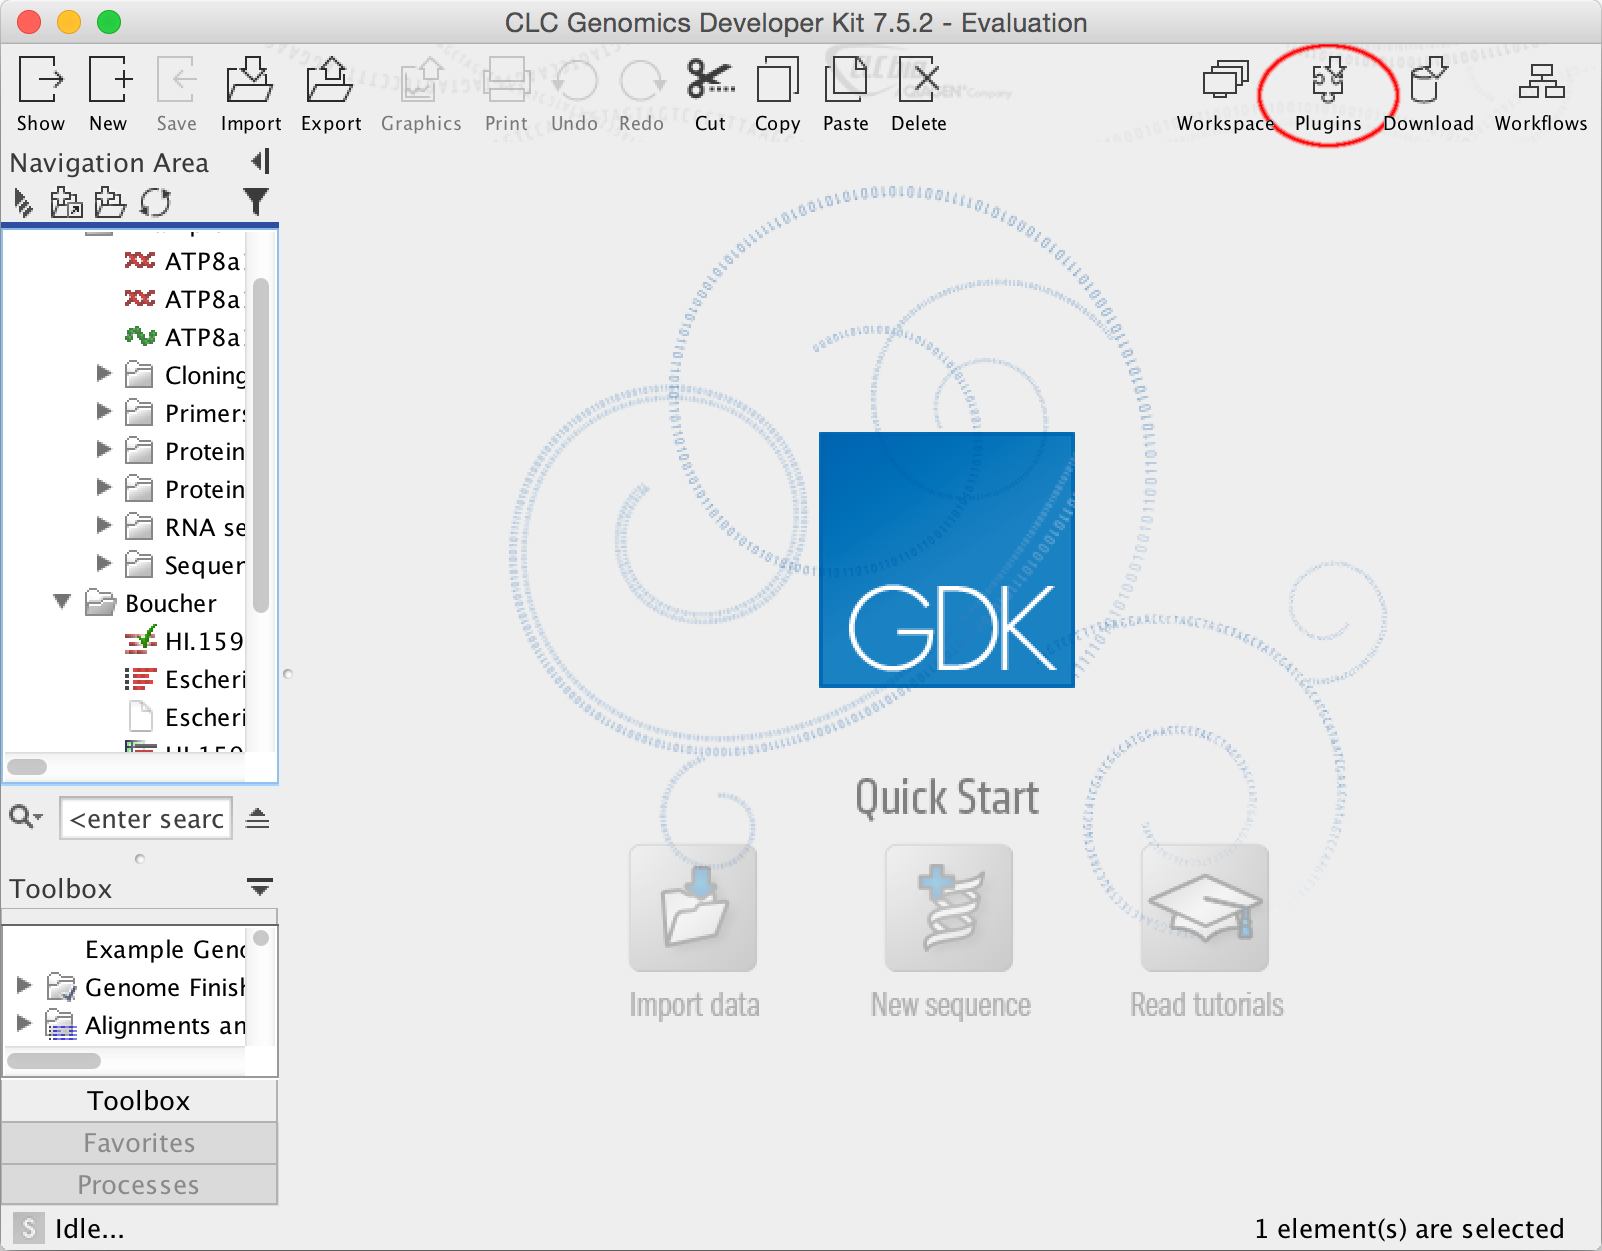
\includegraphics[width=34em]{plugins_button.png}
\end{center}

Then click the \texttt{Install from File} button.

\begin{center}
    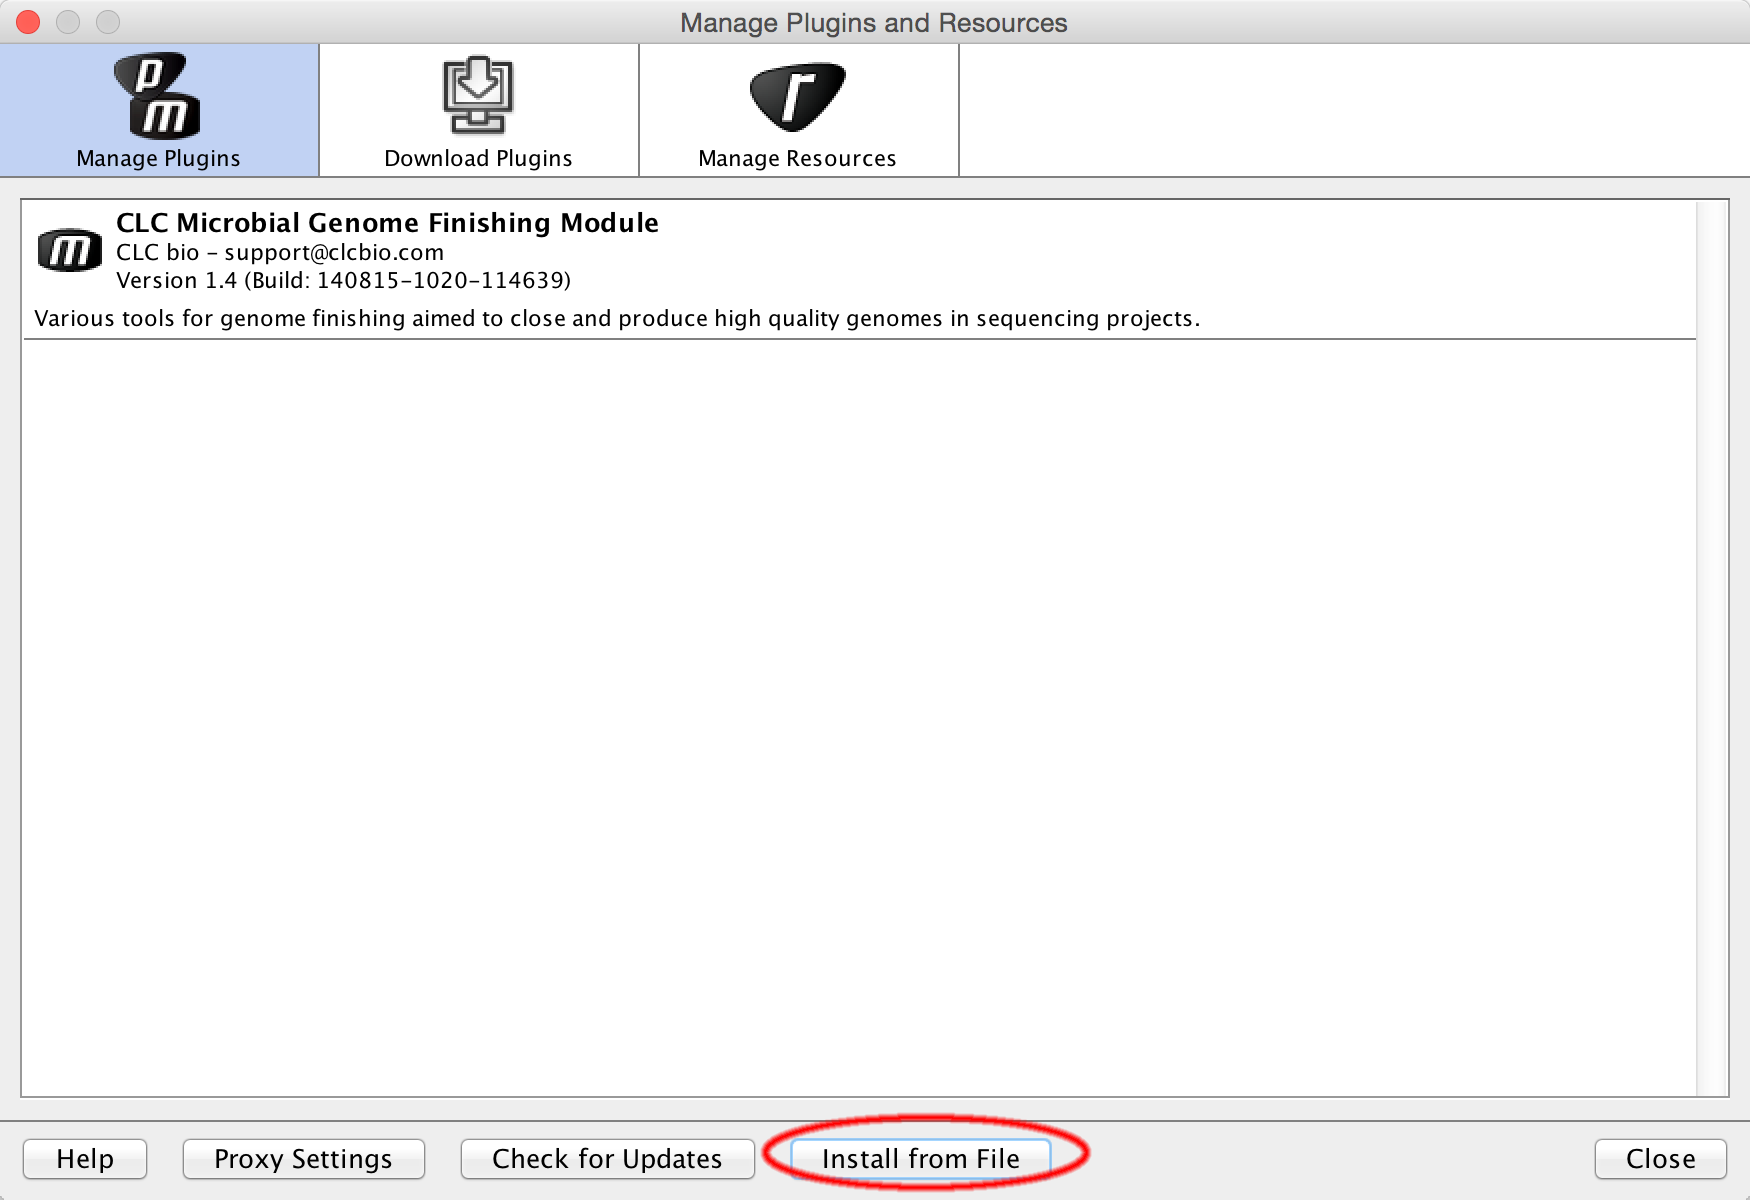
\includegraphics[width=34em]{install_from_file_button.png}
\end{center}

Then navigate to the folder containing the \texttt{ACRD.cpa} file, select the
file, and click the \texttt{Install} button.

\begin{center}
    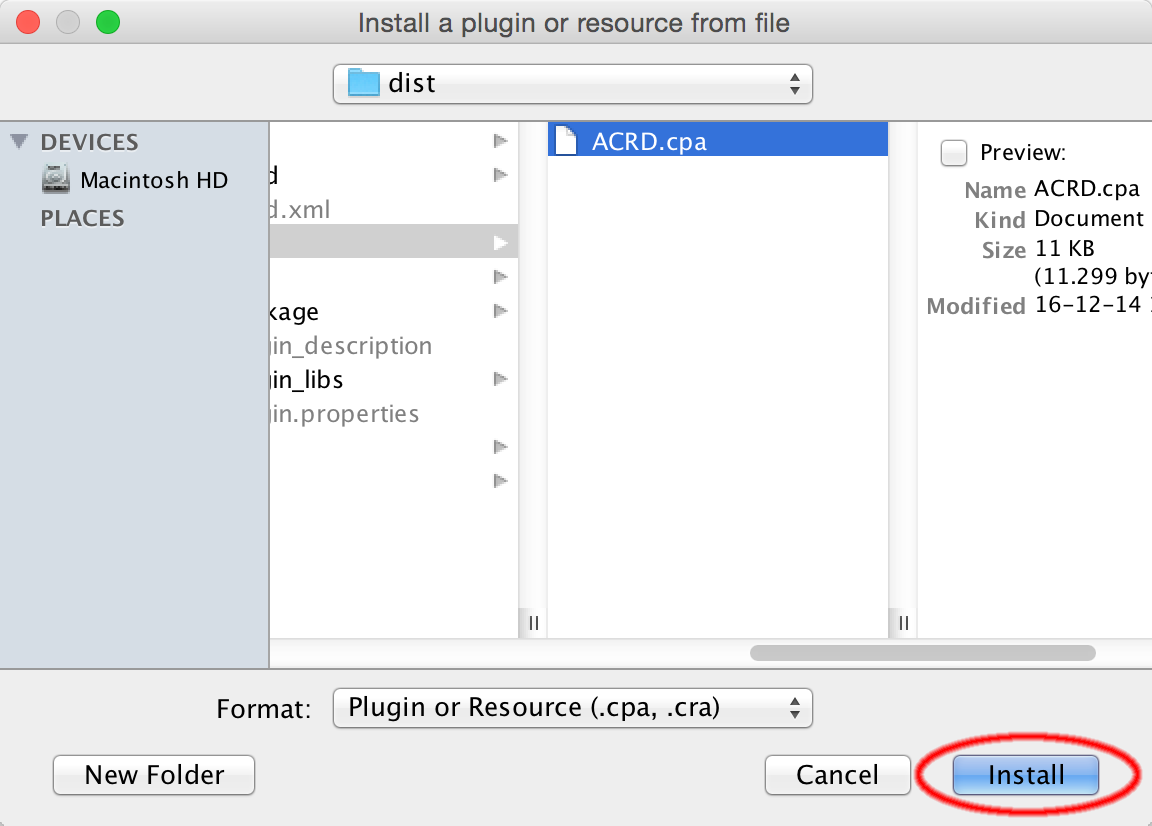
\includegraphics[width=26em]{install_button.png}
\end{center}

Then follow the on-screen steps of the wizard.  CLC Genomics Workbench will
have to be restarted for the plugin to become accessible.

\section{Operation}

\subsection{Data Files}

First, ensure that the necessary data files are available.  ACRD requires two
input files as follows.

\begin{enumerate}
    \item
    The consensus sequence, with the mapped reads.

    \item
    An annotated version of the same consensus sequence.
    \begin{center}
        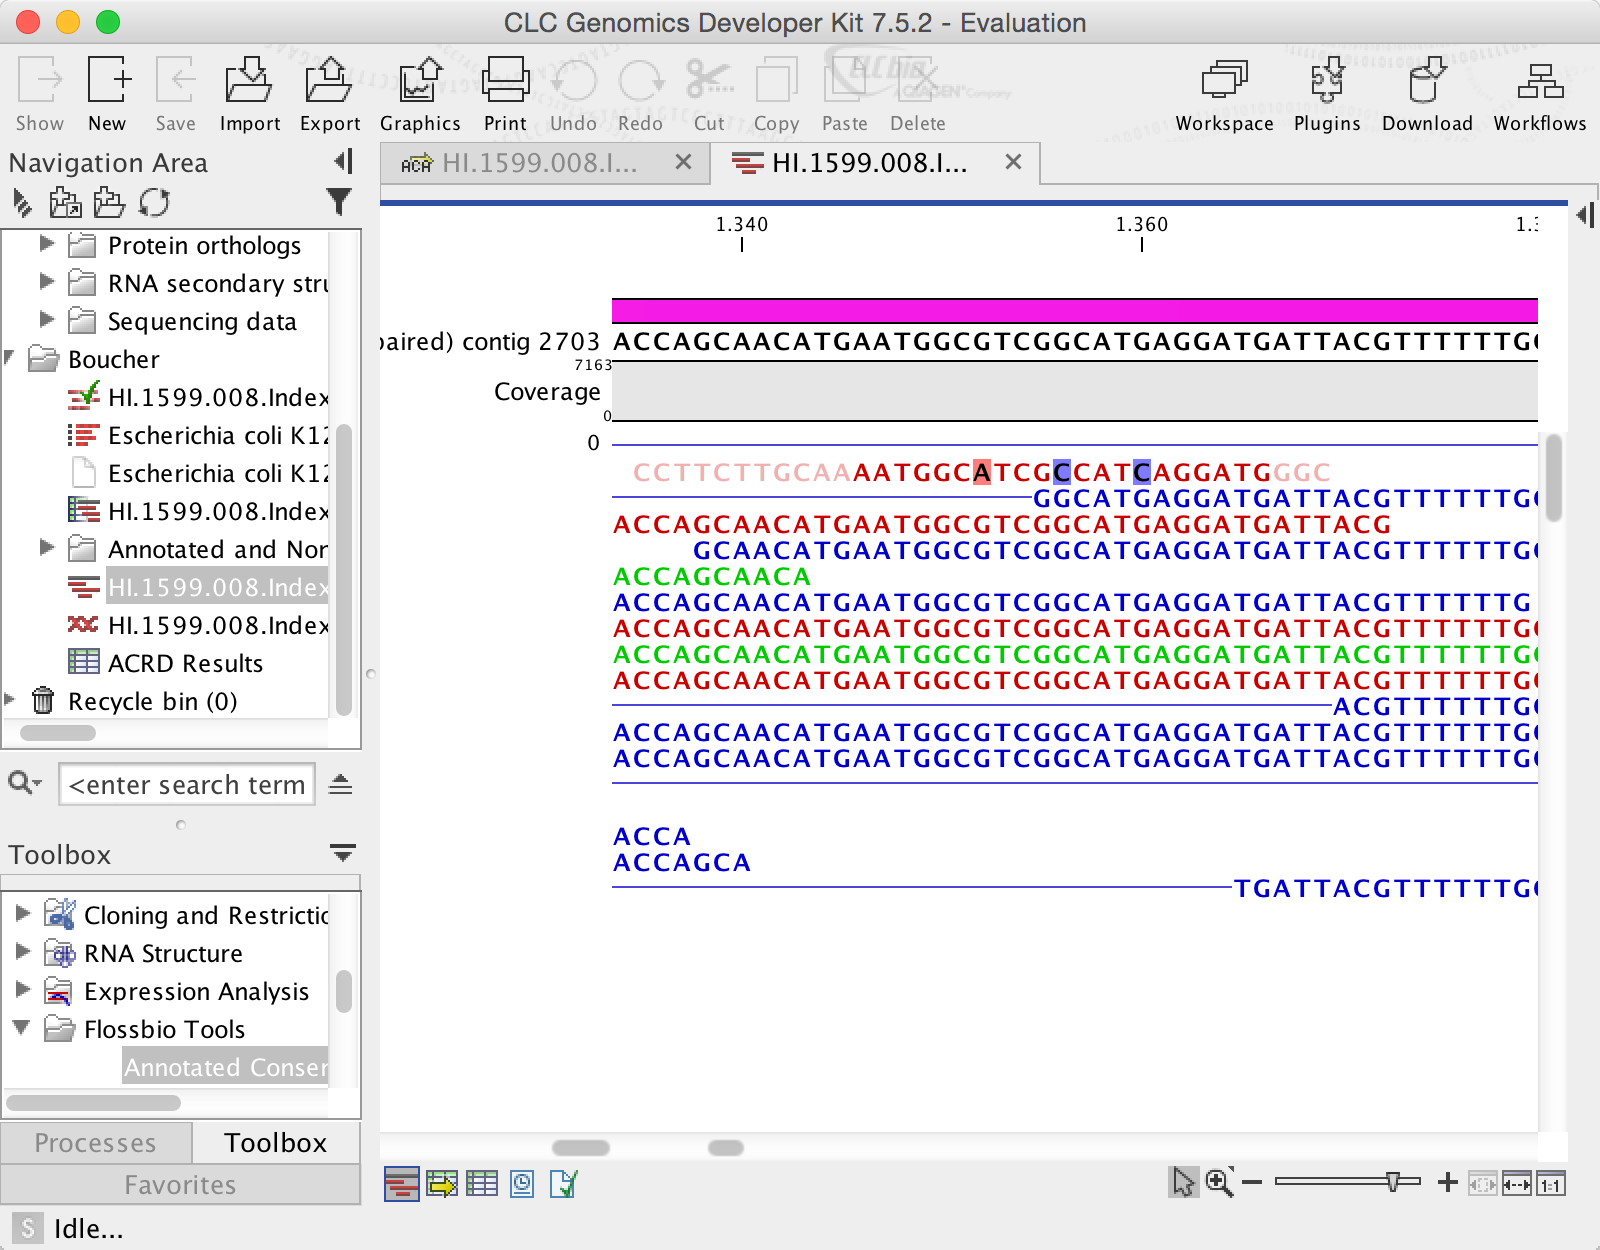
\includegraphics[width=14em]{consensus_mapped_reads.png}
        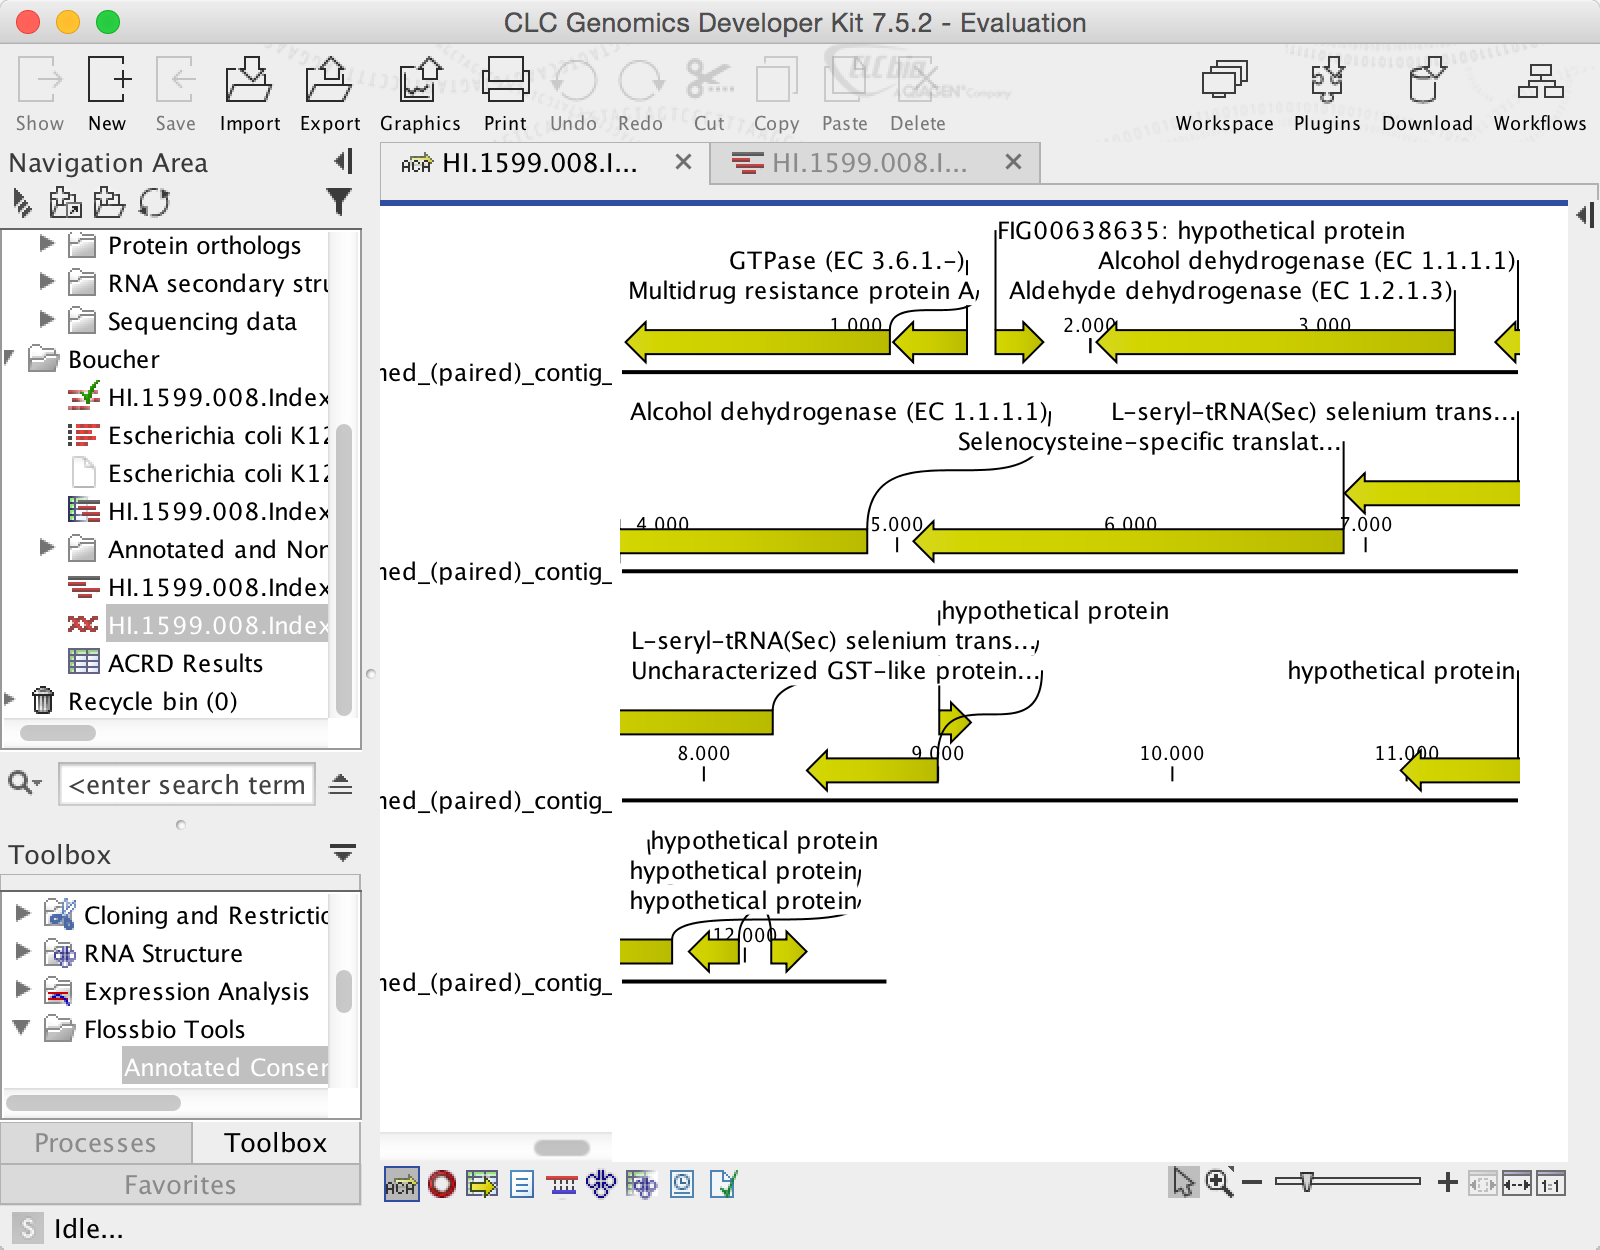
\includegraphics[width=14em]{annotated_sequence.png}
    \end{center}

\end{enumerate}


\subsection{Accessing the Plugin}

In the CLC Genomics Workbench toolbox pane, select \texttt{Flossbio
Tools->Annotated Consensus-Reads Difference} as shown in the following
screenshot.

\begin{center}
    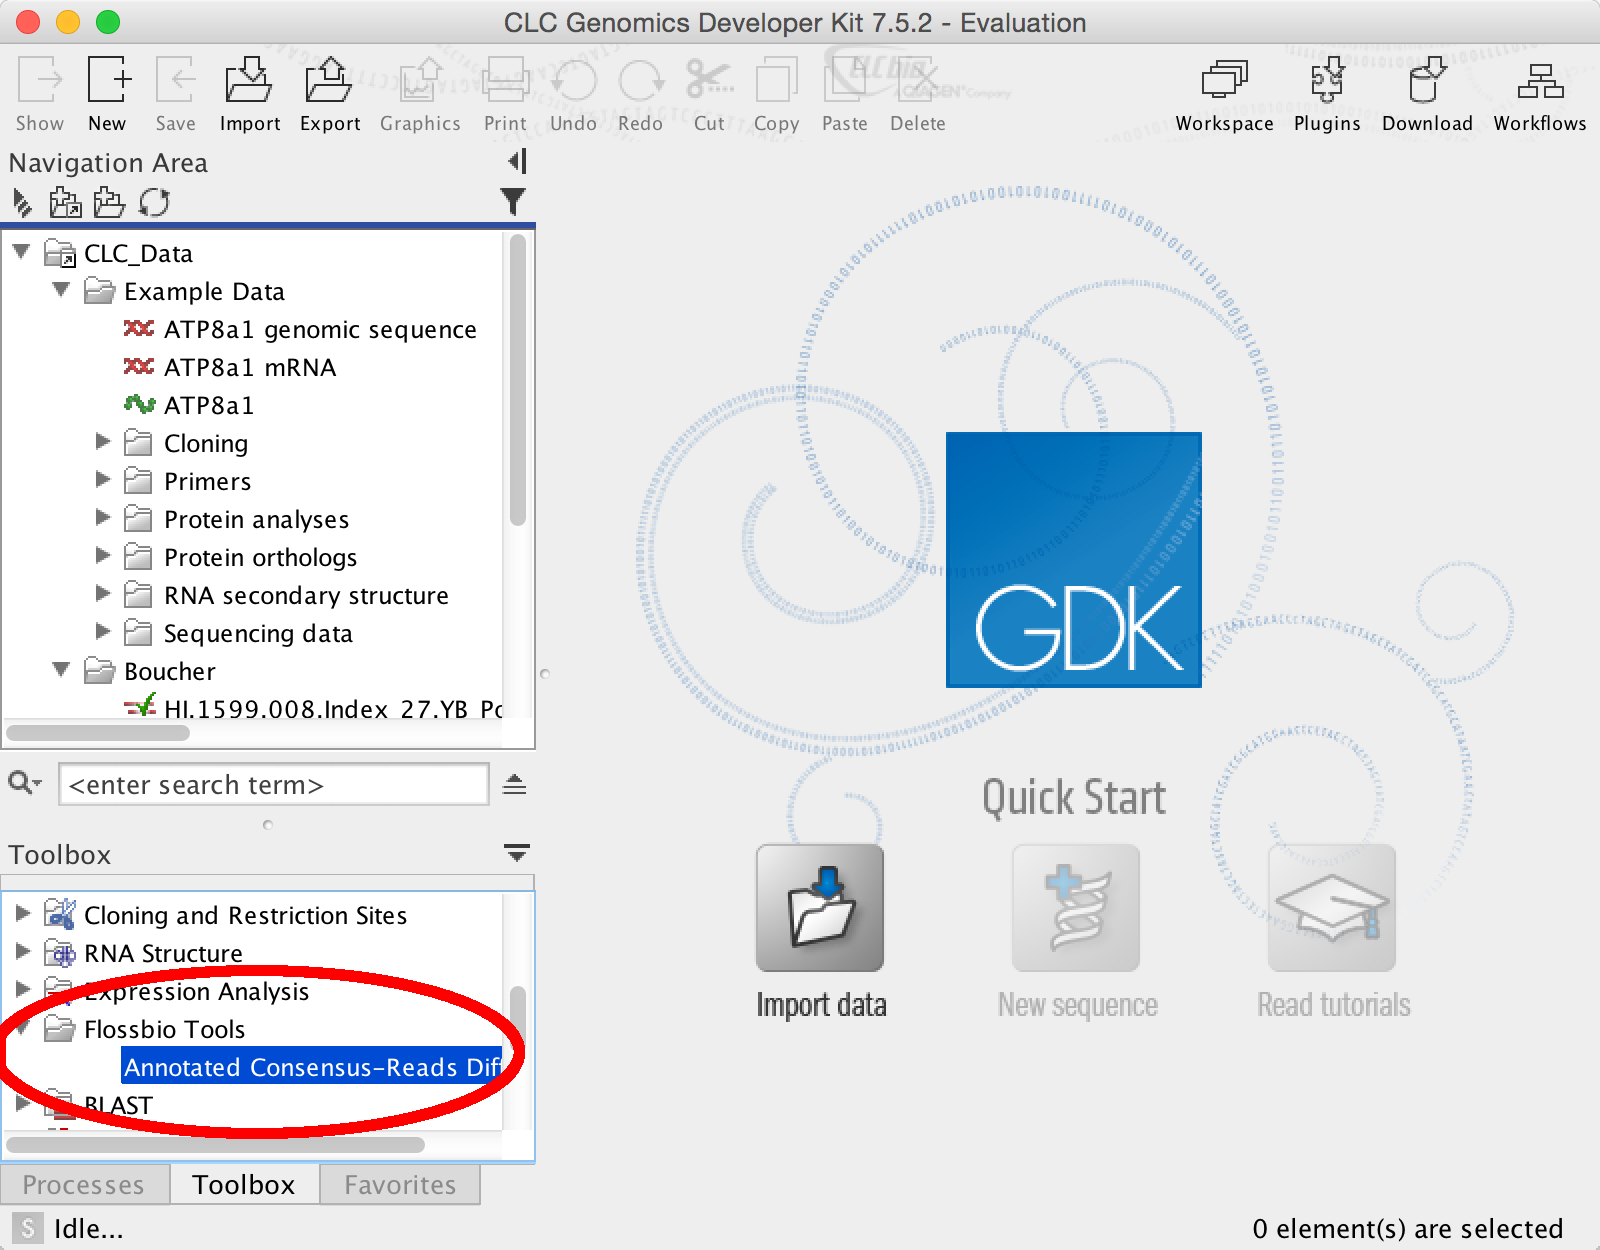
\includegraphics[width=26em]{acrd_toolbox.png}
\end{center}

This will cause an input selection window to open.  Select both the consensus
file with the mapped reads, and the annotated consensus sequence file.

\begin{center}
    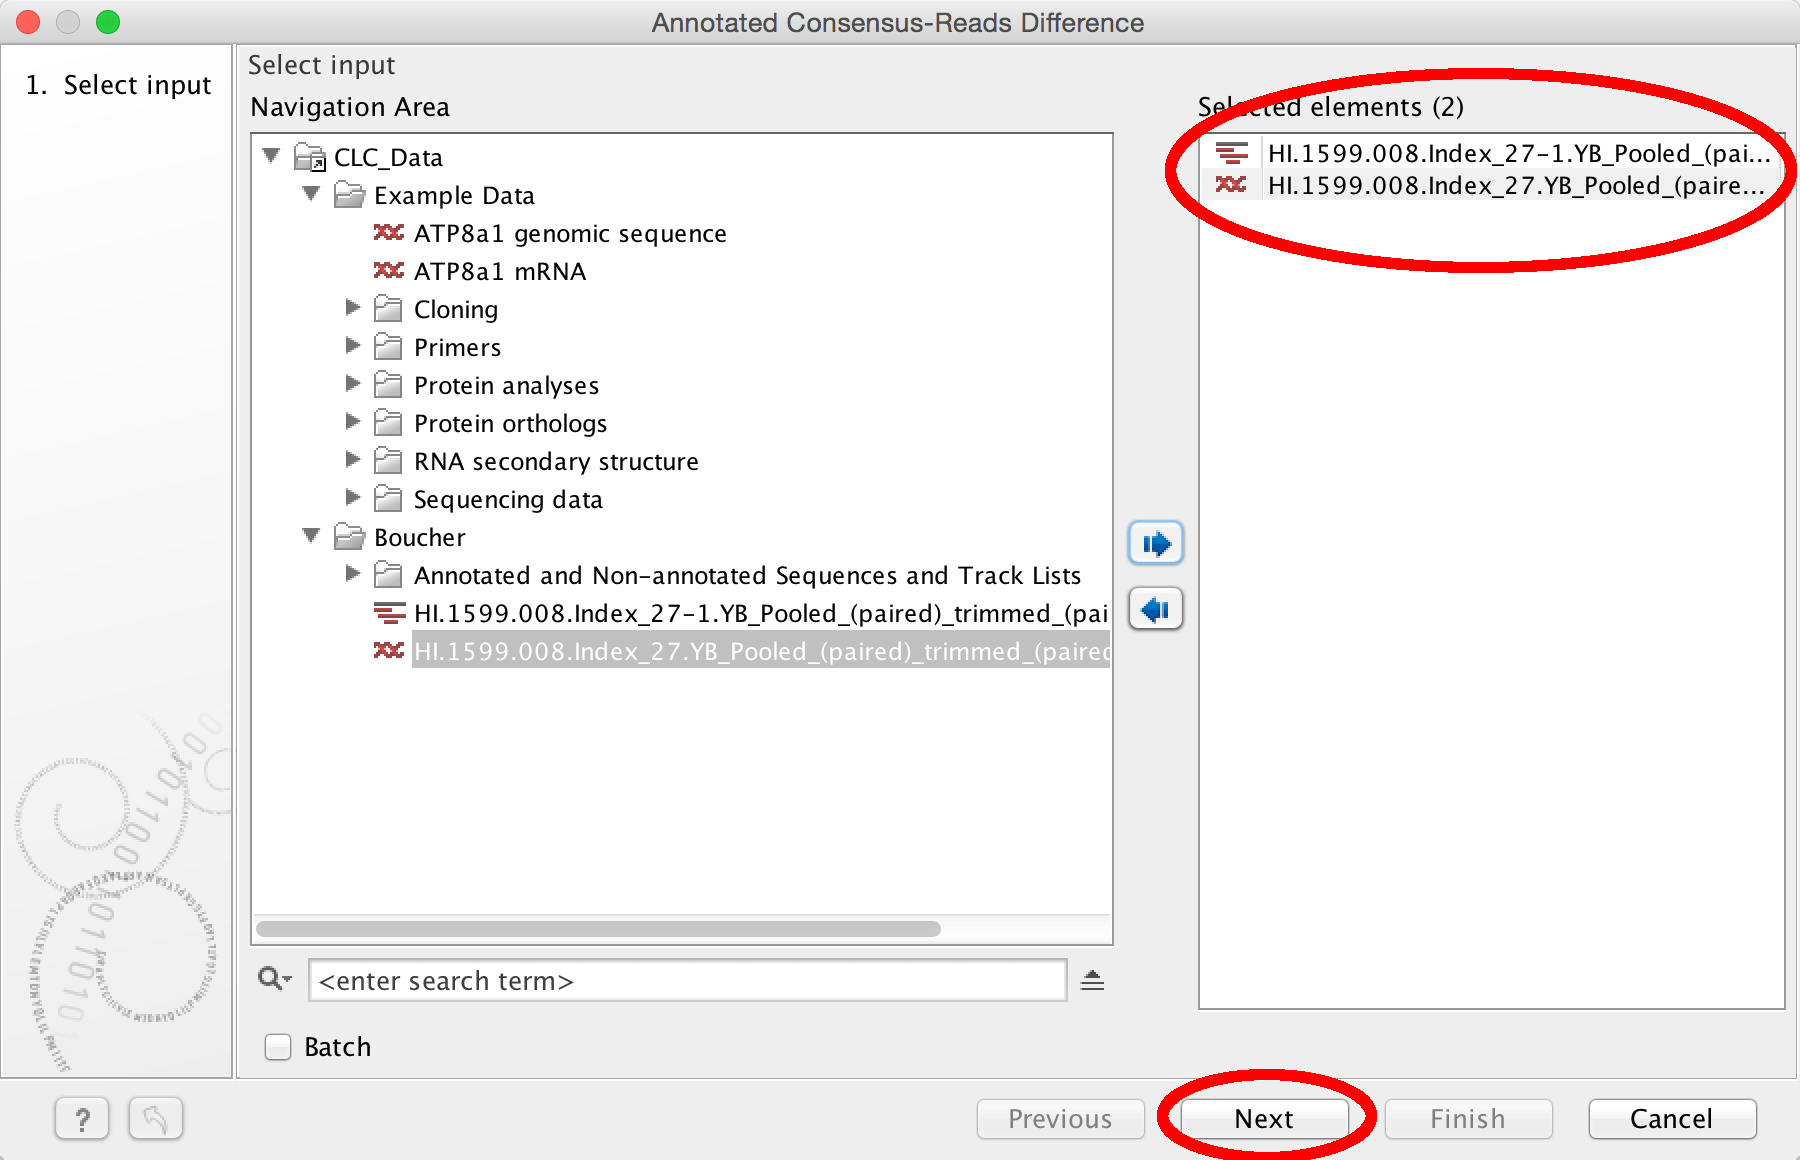
\includegraphics[width=32em]{select_files.png}
\end{center}

After the plugin runs, the resulting analysis will be available, and will look
similar to the following.

\begin{center}
    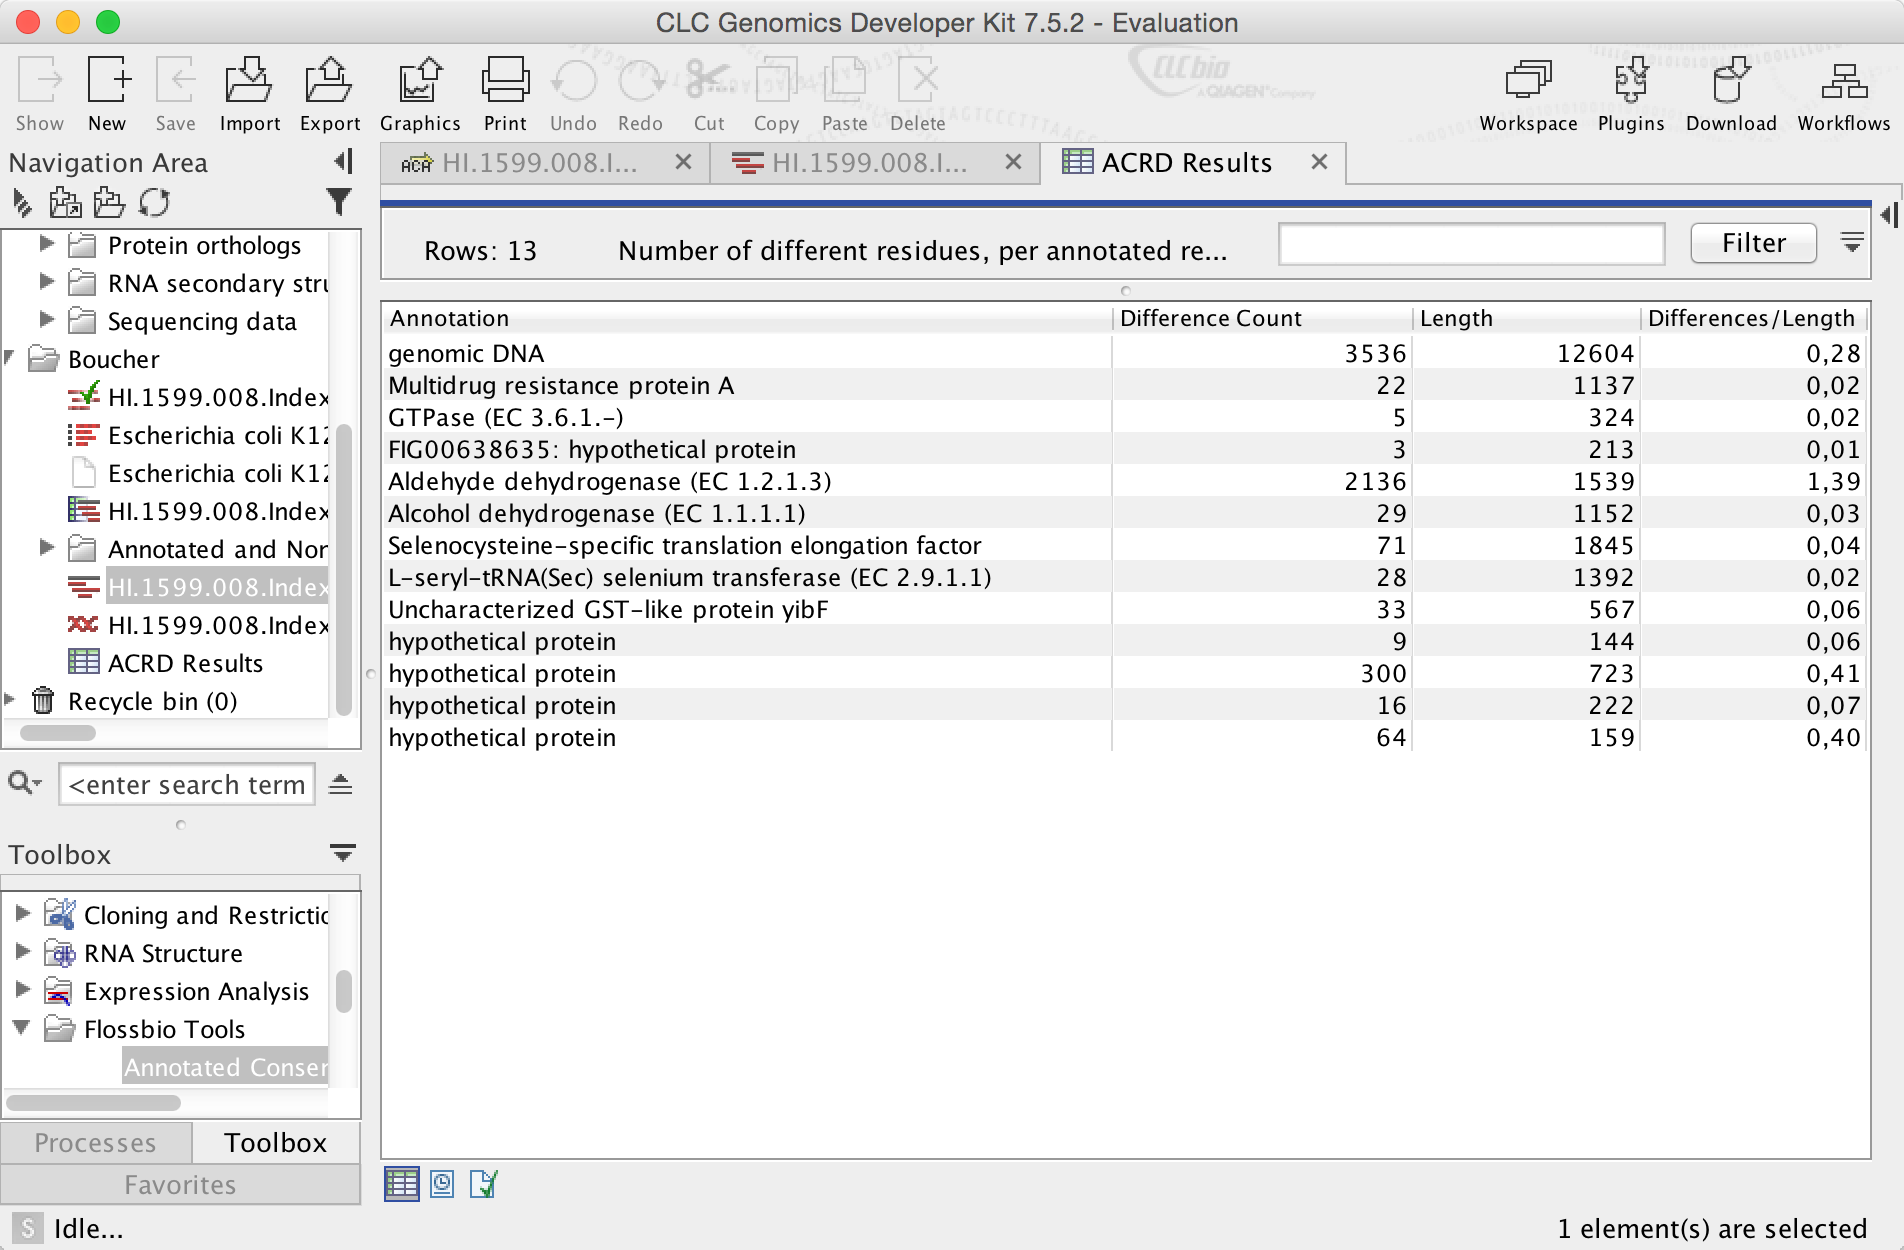
\includegraphics[width=34em]{results.png}
\end{center}

\subsection{Results}

Each row contains the analysis for one annotation.  The first column displays
the name of the annotation.  The second column displays the total number of
differences between read sequences and the consensus sequence inside the
annotated region.  The third column displays the total size of the annotated
region.  The fourth column shows the difference count divided by the length.

\subsubsection{Algorithm Notes}

When counting the differences between the read sequences and the consensus,
mismatching ends of reads are ignored.  So for example, in the left-hand figure
below only four differences are counted because the mismatching head
\texttt{GG} and tail \texttt{GATC} are ignored.

Also, each read is analyzed separately from the others, so all mismatches at
the same location are all counted, even if several of the reads agree with each
other. So for example, in the right-hand figure below five differences are
counted.

\begin{center}
    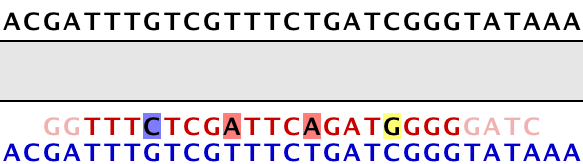
\includegraphics[width=16em]{mismatch_ends_ignored.png}
    \quad
    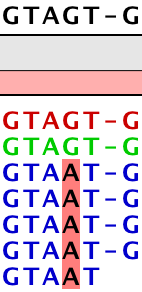
\includegraphics[width=4em]{repeats_all_counted.png}
\end{center}

\section{Additional Information and URLs}

Annotated Consensus-Reads Difference is developed by Jed Barlow at the Boucher
Lab (Department of Biological Sciences, University of Alberta) under the
direction of Yan Boucher.

\begin{itemize}
    \item
        Boucher Lab: \url{http://www.biology.ualberta.ca/boucher\_lab/Boucher\_Lab/Welcome.html}
\end{itemize}

\end{document}
